\chapter{全息张量网络中的算符推移}
\label{chap:operator-pushing}

AdS/CFT 对应\cite{maldacena1999large}中的一项重要特征是在 AdS 体 (bulk) 中演生出的\emph{自由场} (free field)。这使得我们可以为体态提供一套半经典的描述,同时也可以通过体来计算边界 CFT 中的物理量。这里所谓“自由场”,是指其关联函数可以通过 Wick 缩并来计算。一般来说,边界 CFT 中的\emph{单迹算符} (single trace operator) 近似对应了半经典的体态理论中的自由 Gauss 场。这就使得 CFT 中的关联函数可以在 AdS 一侧通过 Witten 图来计算\cite{witten1998anti,gubser1998gauge}。也有很多工作探讨了全息 CFT 中所演生出的广义自由场\cite{dutsch2003generalized,liu2019dimensional,collier2019quantum,nebabu2023bulk}。

另一方面,受 Ryu--Takayanagi 公式\cite{ryu2006holographic}的启发,也有人提出张量网络是构建 CFT 与 AdS 自由度之间线性映射的合适框架\cite{swingle2012entanglement}。如图~\ref{fig:mera-ads-cft} 所示,这类张量网络的图形表示也和 AdS 空间的离散版本非常相似。它描述了 CFT 边界自由度的重整化(粗粒近似)过程,而这些自由度同时也位于张量网络的渐进边界。体中的算符作用在张量网络的辅助指标上,而 CFT 中的算符则作用在张量网络的渐进边界上。因此,张量网络提供了这些算符之间的线性映射\cite{pastawski2015holographic,hayden2016holographic}。

\begin{figure}[htb]
  \centering
  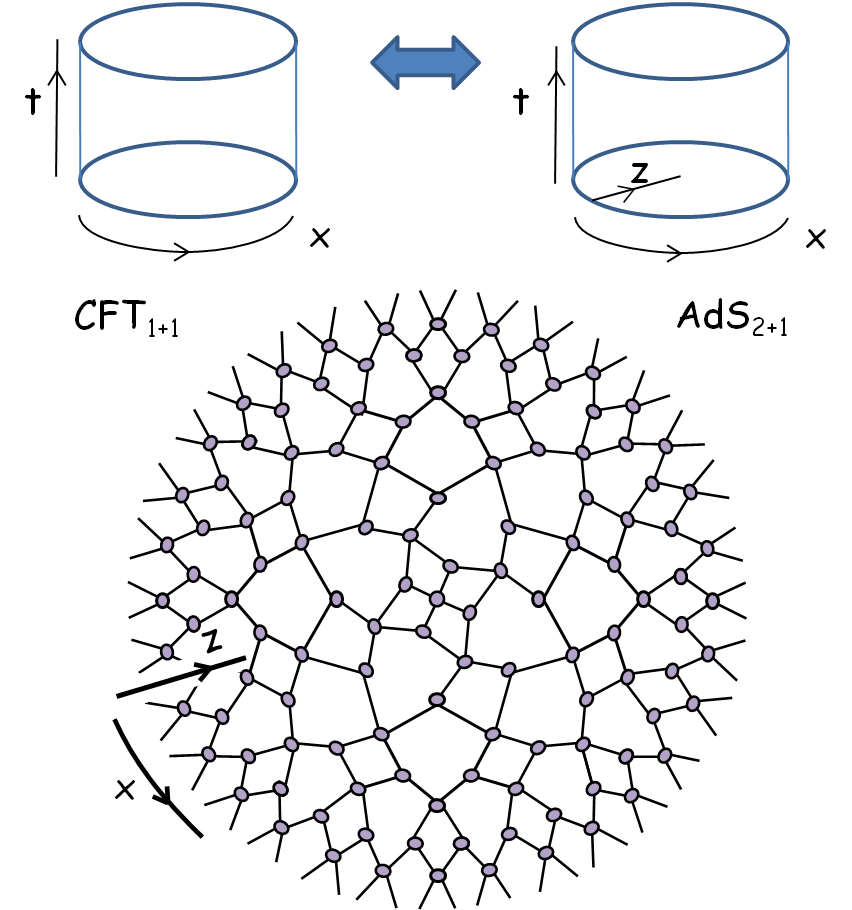
\includegraphics[width=0.5\textwidth]{images/temp/mera-ads-cft.pdf}
  \caption[MERA 张量网络与 AdS/CFT]{MERA 张量网络可以被理解为 AdS/CFT 的一种离散实现。一维格点模型的基态波函数对应了 $\text{CFT}_{1+1}$ 的真空态,而由此“生长”出的二维 MERA 张量网络则给出了 $\text{AdS}_{2+1}$ 时间切片的一种离散表示。图片来源:\parencite{evenbly2011tensor}。}
  \label{fig:mera-ads-cft}
\end{figure}

由于张量网络实际上是局域化的,它可以分解为一系列张量的乘积,而这些张量只与邻近的张量相缩并(邻近张量的具体数目取决于体空间的维数),因而我们可以通过\emph{算符推移} (operator pushing) 的方法来找出相应的\emph{体—边映射} (bulk-boundary map)\cite{pastawski2015holographic,bhattacharyya2016exploring,bhattacharyya2018tensor}。

于是这就引出了一个自然的问题:对于一个弱耦合的体理论,其中的场几乎都是自由的,那么此时什么样的张量网络最能描述相应 AdS/CFT 中的体—边映射?文献 \parencite{bhattacharyya2018tensor} 对这个问题进行了一些讨论。如图~\ref{fig:operator-pushing} 所示,对于体中的算符 $\mathcal{O}$,它作用在体内部的自由度上;而当利用算符推移把 $\mathcal{O}$ 拉到边界时,这种作用应当等价于另一组算符 $\mathcal{O}'$ 在边界自由度上的作用。在利用边界算符对体算符进行重建时,我们有必要对入射、出射腿的方向做出选择。事实上,当张量网络对应了重整化(粗粒近似)操作时,这种选择是唯一的:作用在粗粒近似后的自由度上的算符,应当由作用在粗粒近似前的自由度上的算符来决定。此时可以证明,一个广义的自由场在利用算符推移穿过张量网络后,可以被分解为一系列\emph{简单算符} (simple operators) 之和\cite{bhattacharyya2018tensor}。

\begin{figure}[htb]
  \centering
  % 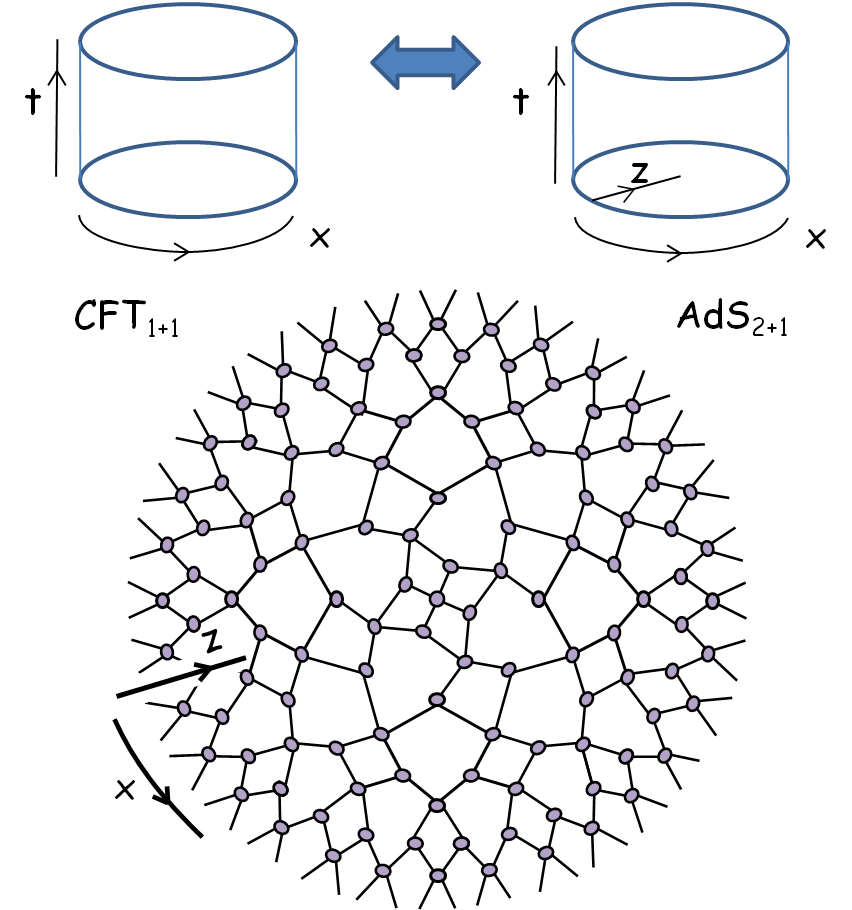
\includegraphics[width=0.5\textwidth]{images/temp/mera-ads-cft.pdf}
  \caption{算符推移}
  \label{fig:operator-pushing}
\end{figure}

考虑一个由重整化张量 $M^{i_1,\dots,i_K}_{j_1,\dots,j_H}\colon\mathbb{V}^K\to\mathbb{V}^H$ 构成的张量网络,其中 $K>H$,$i_l,j_l\in\mathbb{V}$,而 $\mathbb{V}$ 是一个 $d$ 维向量空间。那么算符推移对应于
\begin{equation}
  \mathcal{O} \bigl( \mathbb{V}^H \bigr) \cdot M = M \cdot \mathcal{O} \bigl( \mathbb{V}^K \bigr).
  \label{eq:operator-pushing}
\end{equation}
一个近似自由的体算符会作用在 $\mathbb{V}^H$ 其中一个指标上,即
\begin{equation}
    \mathcal{O} \bigl( \mathbb{V}^H \bigr)
  = \mathbb{I}_1 \otimes \cdots \otimes \mathbb{I}_{i-1} \otimes X_i \otimes \mathbb{I}_{i+1} \otimes \dots \otimes \mathbb{I}_{H}.
\end{equation}
当 $\mathcal{O}$ 满足式~\eqref{eq:operator-pushing} 时,则有
\begin{equation}
    \mathcal{O} \bigl( \mathbb{V}^K \bigr)
  = \sum_{i=1}^K \alpha_i \, \bigl(
      \mathbb{I}_1 \otimes \cdots \otimes \mathbb{I}_{i-1} \otimes X_i \otimes \mathbb{I}_{i+1} \otimes \dots \otimes \mathbb{I}_{K}
    \bigr),
  \label{eq:operator-pushing-coefficients}
\end{equation}
其中 $\{\alpha_i\}$ 为常数。此时,作用在体自由度 $l_B$ 上的体算符 $\mathcal{O}(l_B)$ 就可以用边界算符重建出来:
\begin{equation}
  \mathcal{O} \bigl( l_B \bigr) = \sum_b K^I \bigl( l_b, l_B \bigr) \, \mathcal{O}^I \bigl( l_b \bigr),
\end{equation}
其中 $\{\mathcal{O}^I\}$ 是作用在边界自由度 $l_b$ 上算符的一组完备基,而 $K^I(l_b, l_B)$ 是\emph{体—边核} (bulk-boundary kernel),它可用式~\eqref{eq:operator-pushing-coefficients} 中的系数 $\alpha_i$ 表示。可以发现,这一表达式与通过\emph{体—边传播子} (bulk-boundary propagator) 构造的 \emph{HKLL 核} (HKLL kernel)\cite{hamilton2006local,hamilton2006holographic}具有相同的形式。此外还可以证明,体算符关联函数的行为与广义自由场是类似的\cite{bhattacharyya2018tensor,hung2019padic}。由于 $M$ 是一个长方形的矩阵,所以这种重建不是唯一的。然而,只要式~\eqref{eq:operator-pushing-coefficients} 成立,那么广义自由场的解总是存在的。

\section{1+1 维中的算符推移}

我们首先讨论 1+1 维的情形,即由有限群 $G$ 所描述的 Dijkgraaf--Witten 理论。

\subsection{Abel 的例子:\texorpdfstring{$\mathbb{Z}_n$}{ℤₙ} 群}

\subsection{非 Abel 的例子:\texorpdfstring{$S_3$}{𝑆₃} 群}

\subsection{例子:\texorpdfstring{$\mathbb{Z}_n$}{ℤₙ} 模型}

\subsection{例子:Fibonacci 模型}

\section{本章小结}
